% !TEX root = main.tex
%%%%%%%%%%%%%%%%%%%%%%%%%%%%%%%%%%%%%%%%
%%%%%%%%%%%%%%%%%%%%%%%%%%%%%%%%%%%%%%%%
\section{Results Discussion} \label{sec:results}
%%%%%%%%%%%%%%%%%%%%%%%%%%%%%%%%%%%%%%%%
%%%%%%%%%%%%%%%%%%%%%%%%%%%%%%%%%%%%%%%%

We discuss the achieved results by research question.


\subsubsection{RQ$_{1}$: Injecting a single log statement}
\label{sec:rq1}

\tabref{tab:single-train-results} reports the results achieved by \approach and LANCE, in terms of correct and partially correct predictions for the task of single-log injection. For \approach we only report the results when $k=5$, since this is the variant that achieved the best performance (results with $k=1$ and $k=3$ are available in \cite{replication}). The first row of \tabref{tab:single-train-results} shows the percentage of correct predictions by both approaches, which is slightly higher for \approach (+1.8\% of relative improvement, from 26.78\% to 27.26\%). This difference is statistically significant (adj. $p$-value $<$ 0.01) with 1.12 higher odds of obtaining a correct prediction from \approach as compared to LANCE. 

\begin{table}[h!]
  \centering
  \caption{Correct predictions considering the four-dimensional challenges of injecting log statements.}
  \resizebox{.5\textwidth}{!}{
	  \begin{tabular}{cccccrrrr}
	  \hline
	  Variable   & Level     & Message   & Position  &  & \multicolumn{1}{c}{LEONID} & \multicolumn{1}{c}{LANCE} & \multicolumn{1}{c}{$p$-value} & \multicolumn{1}{c}{OR}     \\ \hline
	  \ding{51}  & \ding{51} & \ding{51} & \ding{51} &  & 27.26\%                    & 26.78\%                   &                           &                            \\
	  \ding{51}  & -         & -         & -         &  & 76.45\%                    & 77.15\%                   &                           &                            \\ 
	  -          & \ding{51} & -         & -         &  & 73.53\%                    & 74.18\%                   &                           &                            \\
	  -          & -         & \ding{51} & -         &  & 31.55\%                    & 30.16\%                   &                           &                            \\ 
	  -          & -         & -         & \ding{51} &  & 82.35\%                    & 82.28\%                   &                           &                            \\ \hline
	  \ding{51}  & \ding{51} & \ding{55} & \ding{51} &  & 28.14\%                    & 29.86\%                    &                           &                            \\ \hline 
	  
	  \end{tabular}
  }
  \label{tab:single-train-results}
\end{table}




The four subsequent rows report the cases in which one of the four log-statement components (variable, level, message, and position) was correctly predicted (\cmark), independently from whether the other three components were correct or not ($-$). As it can be seen, there is no significant difference in the prediction of the log position, with both techniques correctly predicting it in $\sim$82.3\% of cases. Differences are observed for the log variable and level in favor of LANCE (+1.0\% and +0.9\% relative improvement), and for the log message in favor of \approach (+4.6\% relative improvement). The log message is the part for which we observed the strongest OR among all comparisons. Considering that the only difference between \approach and LANCE is the usage of IR, the improvement in the generation of meaningful log messages we targeted has been at least partially achieved. The latter has, however, a small price to pay in the correct prediction of the log variable and level. Still, for these elements \approach is able to generate a correct prediction in over 73.5\% of cases, while the correct generation of the log message still represents the Achilles' heel of these techniques, with 31.55\% correct predictions achieved by \approach. Thus, we believe that improvements on the log message predictions should be favored even at the expense of losing a bit of prediction capabilities on other elements. 

Digging further into the quality of the generated log messages, \tabref{tab:log-messages-stats} reports the results computed using the four NLP metrics presented in \secref{sec:design} for both models (in bold the best results). All metrics suggest that the log messages generated by \approach are closer to those written by humans. According to our statistical analysis (results in \cite{replication}), all these differences are statistically significant (adj. $p$-value $<$ 0.001) with, however, a negligible effect size. For instance, in a recent study Roy \etal \cite{metricsImprovement} showed that differences in METEOR score lower than 2 points are difficult to perceive for humans. 

In our case, we achieved a 1.75 difference. Thus, while overall our analysis showed some improvement in the log message generation when moving from LANCE to \approach, it is unclear whether this has a practical effect when these tools are used by humans.

\begin{table}[h]
	\vspace{-0.2cm}
	\centering
	\caption{RQ$_1$: Evaluation Metrics on Log Messages: LEONID \emph{vs} LANCE\vspace{-0.3cm}}
	\scriptsize
	\label{tab:log-messages-stats}
	 %\resizebox{.5\textwidth}{!}{
	\begin{tabular}{lrr}
		\toprule
		& {\bf LANCE}  &  {\bf LEONID ($k=5$)} \\\midrule
		BLEU-A \cite{papineni2002bleu}& 31.98 & \bf 35.36\\
			\hspace{0.2cm} BLEU-1 & 47.30  & \bf 50.00\\
			\hspace{0.2cm} BLEU-2 & 36.30  & \bf 39.60\\
			\hspace{0.2cm} BLEU-3 & 33.90  & \bf 35.00\\
			\hspace{0.2cm} BLEU-4 & 31.40  & \bf 32.40\\
		METEOR \cite{meteor} & 58.60  & \bf 60.35 \\
		ROUGE-LCS \cite{lin2004rouge} &  \\
		\hspace{0.2cm} $precision$ & 42.57 & \bf 44.68\\
		\hspace{0.2cm} $recall$ & 44.04 &   \bf 46.01\\
		\hspace{0.2cm} $fmeasure$ & 42.19 &  \bf 44.33\\
		LEVENSHTEIN \cite{levenshtein1966} & 44.02 & \bf 41.85 \\\bottomrule
	\end{tabular} 
	\vspace{-0.2cm}
%}
\end{table}


Also the result of our manual inspection of 300 partially correct predictions by \approach and by LANCE point to a similar story: We found 198 of those generated by \approach (66\%) to report the same information of the target log message, despite being semantically different. The remaining 102 (34\%) predictions, instead, reported a log message completely different from the target one or not meaningful at all. For LANCE, the number of semantically equivalent log messages is slightly lower --- 192 (64\%) --- but inline with that observed for \approach. Examples of different but semantically equivalent log messages generated by \approach are available in our replication package \cite{replication}.


\vspace{0.2cm}
\begin{resultbox}
\textbf{Answer to RQ$_1$.} The 3.6 larger training dataset (as compared to the one by Mastropaolo \etal \cite{mastropaolo2022using}) we used to reproduce LANCE, resulted in a boost in performance when predicting the log message (15.20\% in \cite{mastropaolo2022using} \emph{vs.} 30.16\%). Such a result has been further improved by \approach, which achieves a +4.6\% relative improvement (\ie 31.55\% of correctly generated log messages). All metrics used to assess the quality of the log messages generated by \approach indicate improvements over LANCE. Nonetheless, these improvements are marginal, showing that more research is needed to further improve the automated generation of log messages.
\end{resultbox}




%if we have space put this back
%\begin{figure*}[h]
%	\centering
%	\label{fig:rq1-message-stats}
%	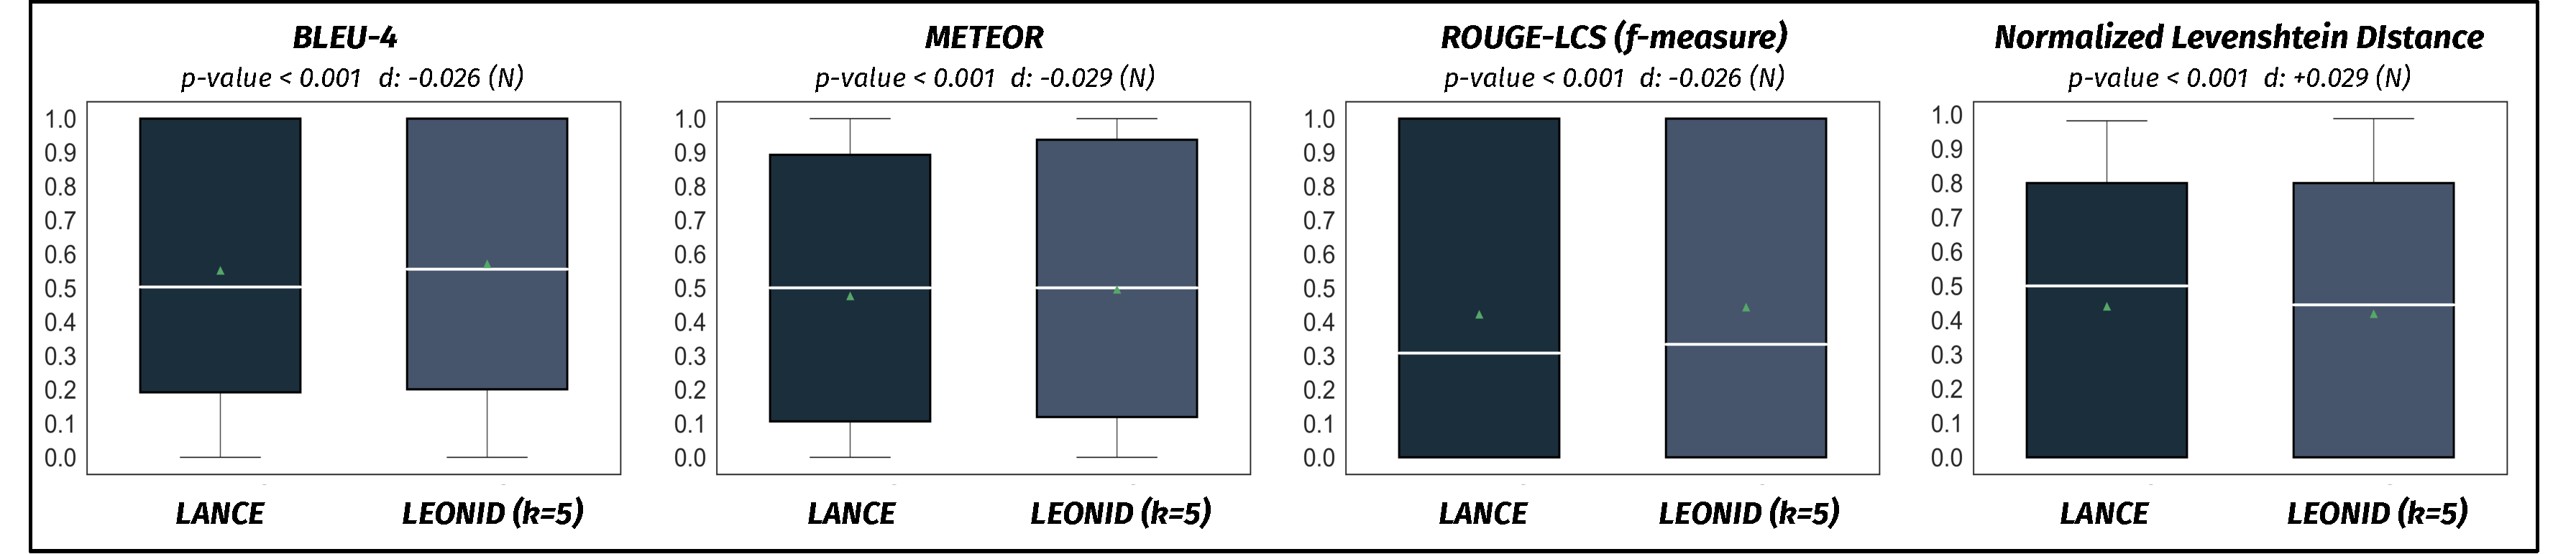
\includegraphics[width=\textwidth]{img/RQ1-log-message-boxplot.pdf}
%	\caption{Characteristics of log messages synthesized by LANCE and LEONID (K=5)}
%\end{figure*}








%\begin{table}[ht]
%	\centering
%	\caption{RQ$_1$: Statistical Tests: LEONID \emph{vs} LANCE for NLP metrics\vspace{-0.3cm}}
%	\scriptsize
%	\label{tab:test-wilcoxon}
%	 \resizebox{.5\textwidth}{!}{
%	\begin{tabular}{llrc}
%		\toprule
%		\textbf{Comparison} & \textbf{Metric} & \textbf{\emph{p}-value} & \textbf{d} \\ 
%		\midrule
%%		\multirow{3}{*}{LANCE  \emph{vs} LEONID ($k=1$)} & BLEU-4 & $<$0.001 & -0.022 (N) \\ 
%%			& METEOR & $<$0.001 & -0.025 (N) \\
%%		& ROUGE-LCS (f-measure) & $<$0.001 & -0.025 (N) \\ 
%%		& LEVENSHTEIN & $<$0.001 & +0.023 (N) \\\midrule
%%		\multirow{3}{*}{LANCE  \emph{vs} LEONID ($k=3$)} & BLEU-4 & $<$0.001 & -0.026 (N) \\ 
%%		& METEOR & $<$0.001 & -0.029 (N) \\
%%		& ROUGE-LCS (f-measure) & $<$0.001 & -0.023 (N) \\ 
%%		& LEVENSHTEIN & $<$0.001 & +0.027 (N) \\\midrule
%			\multirow{4}{*}{LANCE  \emph{vs} LEONID ($k=5$)} & BLEU-4 & $<$0.001 & -0.026 (N) \\ 
%		& METEOR & $<$0.001 & -0.029 (N) \\
%		& ROUGE-LCS (f-measure) & $<$0.001 & -0.026 (N) \\ 
%		& LEVENSHTEIN & $<$0.001 & +0.029 (N) \\\midrule
%	\end{tabular}
%}
%	\vspace{-0.2cm}
%\end{table}


\subsubsection{RQ$_{2}$: Injecting multiple log statements}
\label{sec:rq2}
As explained in \secref{sec:design}, it is not possible to compute the partially correct predictions in the scenario of multiple log injection. Thus, we limit our discussion to the correct predictions generated by \approach. Independently from the value of $k$ (\ie the number of similar coding contexts from which exemplar log messages are extracted), \approach can correctly predict all log statements to inject in a given method in $>$23\% of cases. Also in this scenario, $k=5$ is confirmed as the best configuration, with 23.51\% of correct predictions. Due to space limitations, we provide qualitative examples of correct predictions in our replication package \cite{replication}. 

Interestingly, the drop in performance as compared to the simpler scenario of single log injection is there but is not substantial (27.26\% \emph{vs} 23.51\%). Remember that in this experiment we removed from a given \java method $M$ a random number $y$ of log statements, with $1 \leq y \leq n$ and $n$ being the number of log statements in $M$. Thus, it is possible that most of the methods in our dataset had $n=1$ and, as a consequence, $y=1$ (\ie \approach must generate one log statement), thus making the task similar to the single-log injection. For this reason, we inspected our test set and found indeed that 85\% of methods in it featured, in their original form, a single log statement. On top of this, there is another 6.7\% of methods which originally had more than one log statement and from which we randomly removed $y=1$ statement, thus again resulting in instances requiring the addition of a single log statement. We clustered the instances in the test set based on the number of log statements that \approach was required to generate. We created two subsets: (i) \emph{one-log}, having $y=1$; and (ii) \emph{at-least-two-log}, $y\geq2$. The \emph{one-log} subset features 91.7\% of the instances in the test set (22,104 out of 24,088) and, on those, \approach achieves 24.1\% correct predictions; the \emph{two-log} subset features 1,984 instances (8.3\%), on which \approach has a 17.0\% success rate. Thus, there is an actual performance drop when \approach needs to predict multiple log statements in a given method. Still, in 17\% of cases, \approach is able to inject the same log statements manually written by developers. To give a term of comparison, the original paper presenting LANCE \cite{mastropaolo2022using} reported a 15.2\% success rate for the task of single-log injection.

\vspace{0.2cm}
\begin{resultbox}
\textbf{Answer to RQ$_2$.} \approach can support the task of multiple logs injection, achieving 17.0\% of correct predictions when more than one log statement must be injected. It is worth highlighting how for this task, the model is in charge of inferring how many log statements are actually needed in the method given as input. This makes it a challenging scenario, even when only a single log statement must be injected.
\end{resultbox}

\subsubsection{RQ$_{3}$: Deciding whether log statements are needed}
\label{sec:rq3}

\figref{fig:rq3-cm} reports the confusion matrices for the test sets in \tabref{tab:ds-summary-2}, differing for the proportion of \emph{need}/\emph{no need} instances they feature. Rows in the matrices represent the oracle and columns the predictions. For example, the first matrix to the left indicates that out of the 11,627 (11,013+614) methods in \emph{need} for log statements, \approach correctly identified 11,013 of them, wrongly reporting the remaining 614 as \emph{no need}. Below each matrix we report the overall accuracy of the classifier and the precision and recall for the ``need'' class (\ie when the classifier suggests to add log statements).  

\begin{figure*}[t]
	\centering
	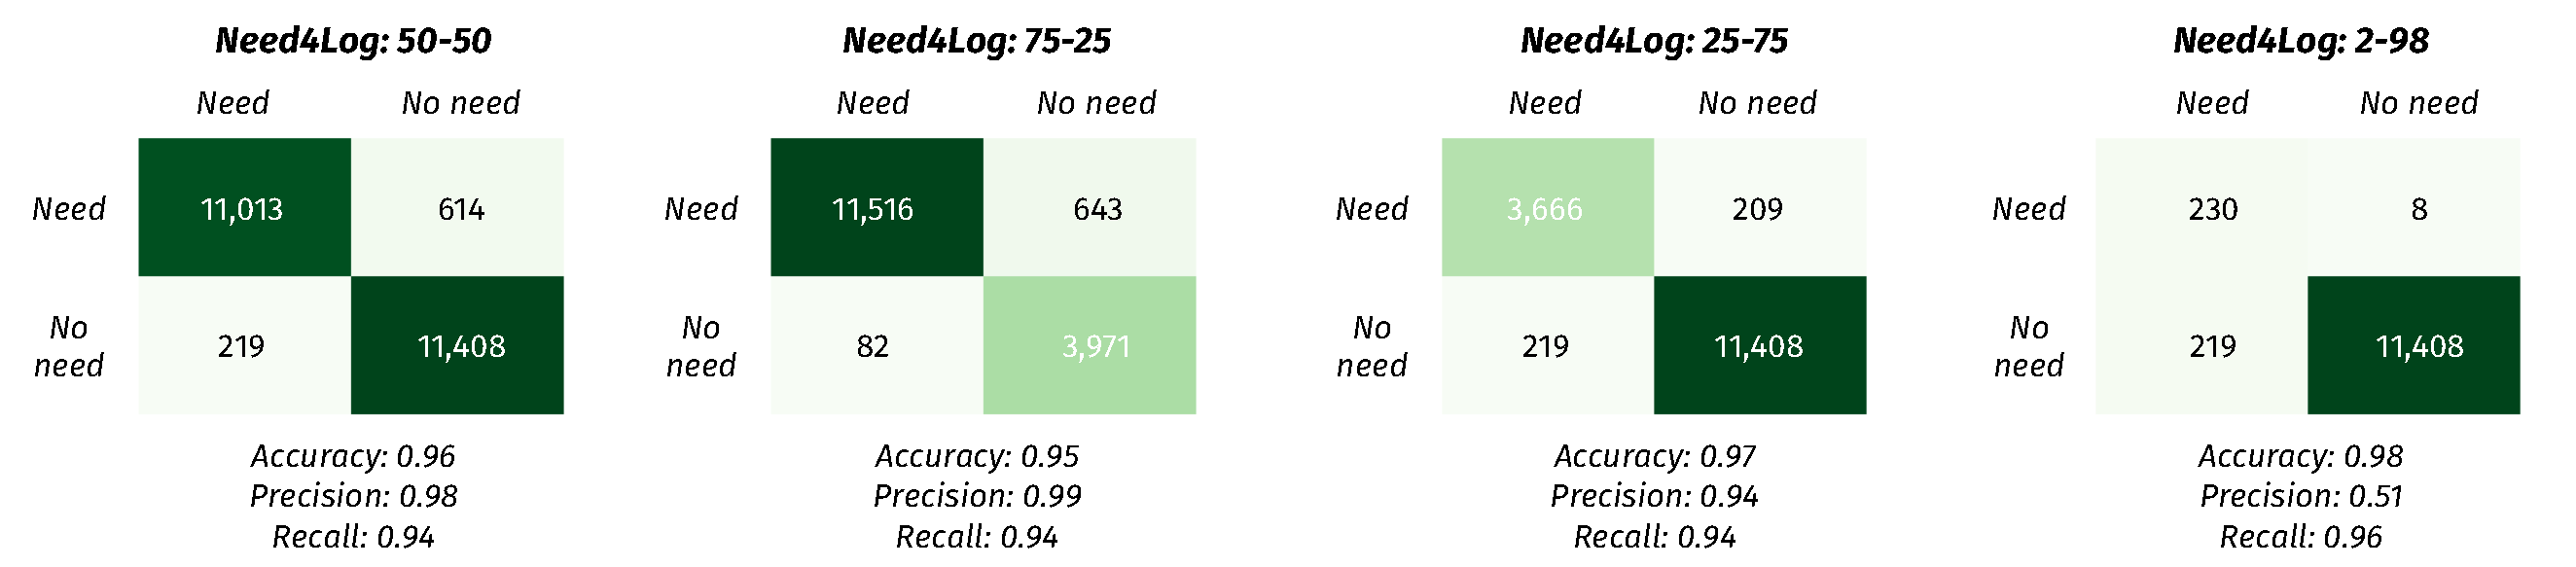
\includegraphics[width=0.8\textwidth]{img/RQ3-CM.pdf}
	\caption{RQ$_3$: Results achieved by \approach when deciding whether log statements are needed or not in \java methods}
	\label{fig:rq3-cm}
	\vspace{-0.3cm}
\end{figure*}

The overall accuracy of the classifier is always very high ($\geq$0.95), indicating that most of instances are correctly classified. Similarly, the recall for the ``need'' class is always $\geq$0.94 (see \figref{fig:rq3-cm}), suggesting that most of the methods in \emph{need} of log statements are identified. 

Instead, the precision drops to 0.51 when the test set is very unbalanced towards the ``no need'' class, with only 238 \emph{need} instances. Indeed, every classification error weights a lot more on the precision when the number of \emph{need} instances is so low: The 219 misclassifications represent 49\% --- 219/(230+219) --- of the instances that \approach classifies as in \emph{need} of log statements. Given the overall very good performance achieved by \approach, we decided to inspect these 219 instances to understand the rationale behind the recommendation by \approach (\ie add log statements). What we found is that, indeed, these are cases which are worth the attention of the developers since they may benefit from additional logging. 

\begin{figure}[h!]
	\centering
	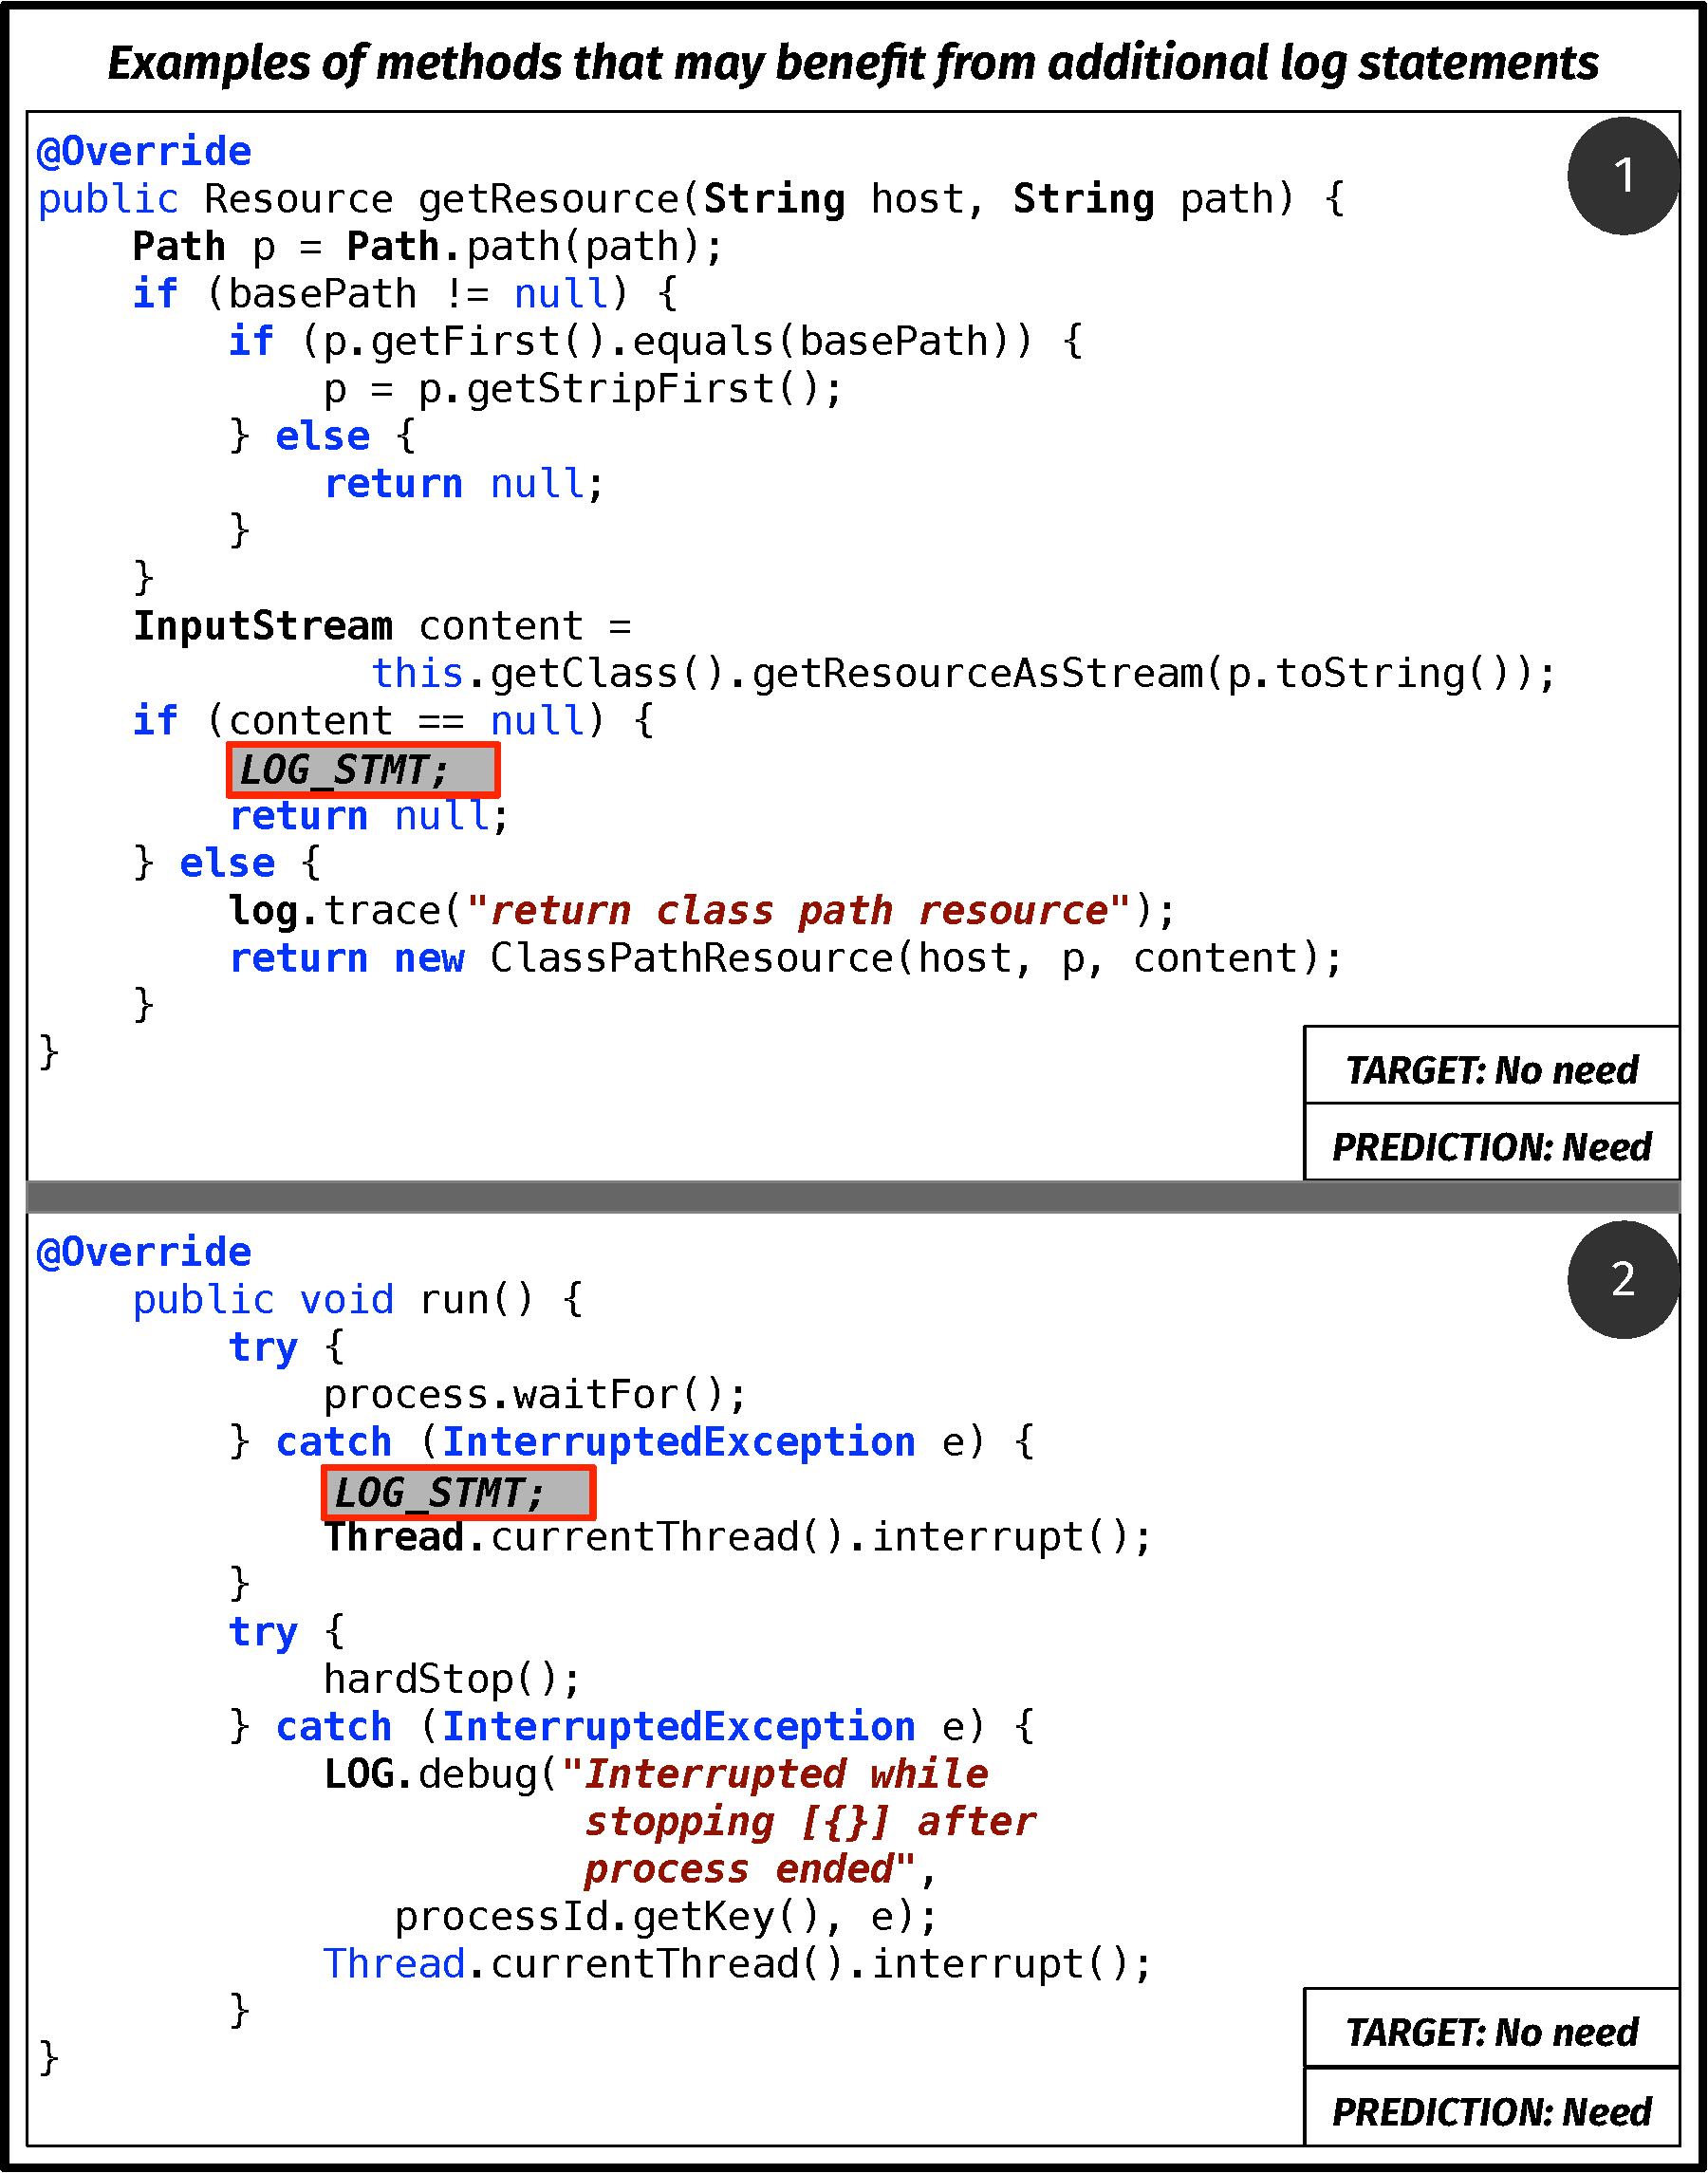
\includegraphics[width=0.85\columnwidth]{img/2-98-examples.pdf}
	\vspace{-0.2cm}
	\caption{Examples of ``\emph{no need} instances'' classified as in \emph{need} for logging}
	\label{fig:no-need}
	\vspace{-0.3cm}
\end{figure}

\figref{fig:no-need} shows two examples of ``\emph{no need} methods'' classified by \approach as in \emph{need} for additional log statements. We added the \emph{LOG\_STMT} text bordered in red to indicate positions which may benefit of logging, especially considering the other log statements present in the method. For example, in method \texttt{run} \circled{2} the developers used a log statement to document the reason for the \texttt{InterruptedException} in the second \texttt{try/catch}, while a similar scenario in the first \texttt{try/catch} is not logged. Overall, based on our manual inspection of the ``false positives'', we are confident that these could still represent valuable recommendations for developers.

Finally, when comparing the correct predictions achieved by \approach with those of the optimistic, pessimistic, and random classifier, we always found a statistically significant difference in favor of \approach (adj. $p$-value $<$ 0.001) accompanied by an OR going from a minimum of 6.17 to a maximum of 1,426. The only exception is, as expected, the comparison with the pessimistic classifier on the 2-98 test set, on which the pessimistic classifier achieves 98\% of correct predictions. In this case, we found no statistically significant difference (adj. $p$-value $=$ 0.63) with \approach (detailed results in \cite{replication}).

\vspace{0.2cm}
\begin{resultbox}
\textbf{Answer to RQ$_3$.} \approach can discriminate between methods \emph{needing} and \emph{not needing} additional log statements, with an accuracy higher than 0.95. Our results suggest that this binary classifier can be used as a preliminary step before running, when needed, models aimed at injecting log statements.
\end{resultbox}

%\begin{table}[ht]
%	\centering
%	\caption{Statistical Tests: LEONID \emph{vs} NAIVE Classifiers\vspace{-0.2cm}}
%	\scriptsize
%	\label{tab:statistical-classifier}
%	\resizebox{.5\textwidth}{!}{
%		\begin{tabular}{llrc}
%			\toprule
%			\textbf{Test Set} & \textbf{Metric} & \textbf{\emph{p}-value} & \textbf{OR} \\ 
%			\midrule
%			\multirow{3}{*}{Need4Log: (50-50)} 
%			& Optimistic \emph{vs} LEONID & $<$0.001 &18.57 \\ 
%			& Pessimistic \emph{vs} LEONID & $<$0.001 & 50.28 \\ 
%			& Random \emph{vs} LEONID & $<$0.001 & 27.12 \\\midrule
%			\multirow{3}{*}{Need4Log: (75-25)} 
%			& Optimistic \emph{vs} LEONID & $<$0.001 & 6.17 \\ 
%			& Pessimistic \emph{vs} LEONID & $<$0.001 & 140.43 \\ 
%			& Random \emph{vs} LEONID & $<$0.001 & 21.41 \\\midrule
%			\multirow{3}{*}{Need4Log: (25-75)} 
%			& Optimistic \emph{vs} LEONID & $<$0.001 & 54.58 \\ 
%			& Pessimistic \emph{vs} LEONID & $<$0.001 & 16.73 \\ 
%			& Random \emph{vs} LEONID & $<$0.001 & 33.77 \\\midrule
%			\multirow{3}{*}{Need4Log: (2-98)} 
%			& Optimistic \emph{vs} LEONID & $<$0.001 & 1,426 \\ 
%			& Pessimistic \emph{vs} LEONID & 0.63 & 1.05 \\ 
%			& Random \emph{vs} LEONID & $<$0.001 & 56.53 \\\midrule
%		\end{tabular}
%	}
%	\vspace{-0.2cm}
%\end{table}





%complementarity
%Shared:  72.05602393255371
%Only LEONID:  14.781071525700298
%Only LANCE:  13.162904541745988

